\section{Results}
\label{sec:results}

\subsection{Setup}

All benchmarks ran on an AMD Ryzen 5 7640HS (6 cores, 12 threads), 12\,GiB DDR5, NVMe SSD, Debian 13, \texttt{rustc} 1.94.0 release mode.
Synthetic references of 1\,MB and 10\,MB were generated with ${\sim}40$\% GC content.
Each configuration ran three times with different seeds.
Mean values are reported.

\subsection{Coverage scaling}

Figure~\ref{fig:cov-scaling} shows wall time and peak memory as a function of coverage depth on the 1\,MB reference with 100 mutations.
Both scale linearly ($R^2 > 0.999$).
Throughput stabilises at ${\sim}13{,}000$ read pairs/s above 10x.
The lower rate at 1x reflects startup overhead.

\begin{figure}[t]
  \centering
  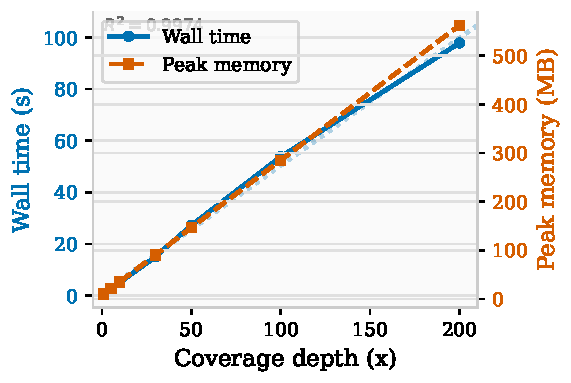
\includegraphics[width=\linewidth]{../../benchmarking/results/graphs/coverage_scaling.pdf}
  \caption{Wall time and peak memory vs coverage depth (1\,MB reference, 100 mutations, 12 threads). Both scale linearly with $R^2 > 0.999$.}
  \label{fig:cov-scaling}
\end{figure}

\subsection{Feature overhead}

Figure~\ref{fig:features} shows the incremental cost of each feature at 30x on the 1\,MB reference (${\sim}200$K read pairs).
Variant injection and GC bias are within measurement noise ($<1$\%).
FFPE/oxoG artefacts add 15\% via a per-base damage pass.
UMI simulation dominates at +143\% due to PCR family tracking across cycles.
The combined overhead of +198\% is super-additive: UMI families must carry variant and artefact state through each PCR cycle, compounding the individual costs.

\begin{figure}[t]
  \centering
  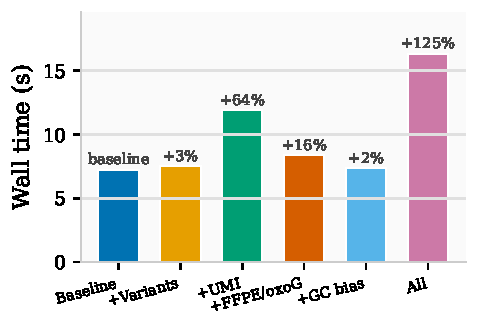
\includegraphics[width=\linewidth]{../../benchmarking/results/graphs/feature_overhead.pdf}
  \caption{Feature overhead relative to baseline (1\,MB, 30x). Variant injection and GC bias are free. FFPE adds 16\%. UMI dominates at +64\%.}
  \label{fig:features}
\end{figure}

\subsection{Throughput}

Table~\ref{tab:scenarios} summarises the main scenarios.
At baseline (10\,MB, 30x, 12 threads), \varforge{} produces ${\sim}2.0$M read pairs in 139.6\,s (${\sim}14{,}300$ pairs/s, ${\sim}4.3$\,Gbp/min).
Adding 500 mutations increases wall time by $<0.1\%$.
Figure~\ref{fig:throughput} compares throughput across scenarios.

\begin{table}[t]
\centering
\caption{Main benchmark scenarios (12 threads, mean of 3 runs).}
\label{tab:scenarios}
\small
\setlength{\tabcolsep}{3.5pt}
\begin{tabular}{@{}llrrlrr@{}}
\toprule
Config & Ref & Cov & Var. & Features & Wall (s) & \makecell{Peak\\RAM (GB)} \\
\midrule
Baseline         & 10\,MB & 30x  & ---  & ---             & 139.6 & 0.87 \\
+Variants        & 10\,MB & 30x  & 500  & ---             & 139.7 & 0.87 \\
High cov (1\,MB) & 1\,MB  & 200x & 100  & ---             &  92.7 & 0.58 \\
cfDNA            & 1\,MB  & 200x & 200  & cfDNA, 2\% pur. &  92.5 & 0.68 \\
FFPE + oxoG      & 10\,MB & 30x  & 500  & artefacts       & 170.5 & 1.17 \\
Panel + UMI      & 1\,MB  & 200x & 50   & UMI simplex     & 195.1 & 1.80 \\
\bottomrule
\end{tabular}
\end{table}

\begin{figure}[t]
  \centering
  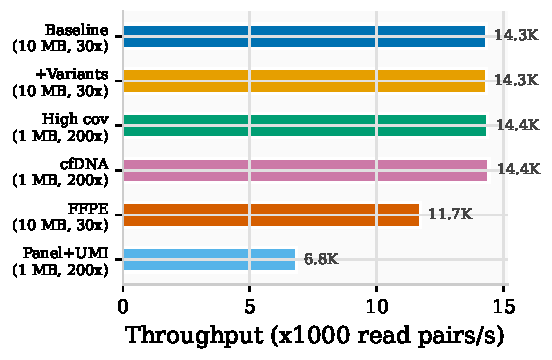
\includegraphics[width=\linewidth]{../../benchmarking/results/graphs/throughput_scenarios.pdf}
  \caption{Throughput across scenarios. All I/O-bound configs converge to ${\sim}13$--$14$K pairs/s. Panel+UMI is lower (${\sim}6{,}800$ pairs/s) due to PCR family tracking overhead.}
  \label{fig:throughput}
\end{figure}

\subsection{Thread scaling}

Figure~\ref{fig:threads} shows scaling on the 10\,MB, 30x configuration.
Adding threads does not improve wall time for this I/O-bound workload.
Single-threaded execution takes 140\,s; 12 threads takes 160\,s, a 13\% regression.
Workers complete their compute work quickly, then contend on the single writer thread draining the channel.
The coordination overhead dominates.
Threading provides value for compute-heavy workloads (UMI simulation) where each worker occupies the CPU longer before writing.
See Section~\ref{sec:discussion} for a discussion of when threading helps.

\begin{figure}[h]
  \centering
  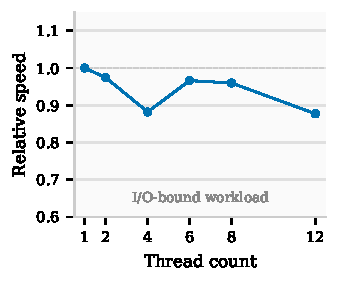
\includegraphics[width=0.45\linewidth]{../../benchmarking/results/graphs/thread_scaling.pdf}
  \caption{Thread scaling (10\,MB, 30x). I/O-bound: adding threads degrades performance by up to 13\%.}
  \label{fig:threads}
\end{figure}

\subsection{hg38 (chr22) benchmarks}

Table~\ref{tab:hg38} reports performance on chromosome~22 from hg38 (${\sim}51$\,Mbp) at 5x coverage.
All six configurations completed.
The coverage was set to 5x rather than clinical depths (500x for panels, 200x for cfDNA) because \varforge{} does not yet support BED-based region filtering; the purpose of these benchmarks is to confirm correct operation on a real reference, not to generate high-coverage datasets (see Section~\ref{sec:future}).
UMI configs (3--4) produce more output read pairs than the baseline because PCR family expansion is included in the output.

\begin{table}[t]
\centering
\caption{hg38 chr22 benchmarks (5x, 1 run each, 12 threads). UMI/duplex configs show higher read counts due to PCR family expansion and higher RAM from family tracking.}
\label{tab:hg38}
\small
\setlength{\tabcolsep}{3.5pt}
\begin{tabular}{@{}llrrrr@{}}
\toprule
\# & Config & Wall (s) & Peak RAM (GB) & Read pairs & Pairs/s \\
\midrule
1 & WGS baseline      &  96.6 & 0.72 &   847K & 8,772 \\
2 & WGS + variants    &  96.6 & 0.72 &   847K & 8,772 \\
3 & Panel UMI simplex & 233.1 & 2.26 & 2,540K & 10,894 \\
4 & Twist duplex      & 298.6 & 3.00 & 3,389K & 11,349 \\
5 & cfDNA liq.~biopsy &  96.6 & 0.85 &   847K & 8,772 \\
6 & FFPE tumour       & 121.1 & 0.91 & 1,059K & 8,746 \\
\bottomrule
\end{tabular}
\end{table}

\subsection{Memory efficiency}

Figure~\ref{fig:mem} shows per-pair memory is constant at ${\sim}0.45$\,KB across coverage depths above 10x.
The streaming architecture bounds peak memory by channel depth and concurrent batch state rather than dataset size.
A full human genome 30x WGS run produces ${\sim}600$M pairs, but only the in-flight batches must reside in memory at any one time, making it feasible on a standard workstation.

\begin{figure}[t]
  \centering
  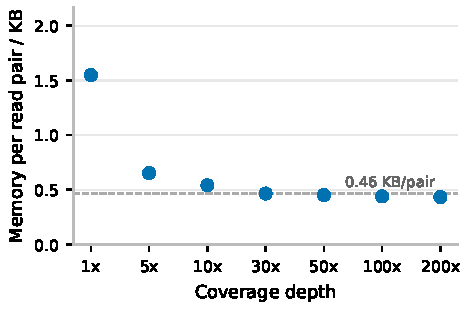
\includegraphics[width=\linewidth]{../../benchmarking/results/graphs/memory_per_pair.pdf}
  \caption{Memory per read pair across coverage depths. The constant ${\sim}1.7$\,KB/pair confirms the streaming architecture bounds memory by batch size, not dataset size.}
  \label{fig:mem}
\end{figure}
